\RequirePackage{luatex85}
\documentclass{standalone}

\usepackage{xparse}

\usepackage{amsmath}
\newcommand{\vectorunit}[1]{\hat{\mathbf{#1}}}
\NewDocumentCommand\norm{ o m }{\|\mathbf{#2}\|\IfNoValueF{#1}{_{#1}}}

\usepackage{fontspec, unicode-math}
\setsansfont[Scale=MatchLowercase]{TeX Gyre Heros}
\setmathfont{TeX Gyre Termes Math}

\usepackage{tikz}
\usetikzlibrary{arrows.meta}
\usepackage{pgfplots}
\pgfplotsset{compat=1.14}

\tikzset{
  every picture/.style={font={\sffamily\normalsize}, >=stealth},
  every pin edge/.style={black}}

\begin{document}

  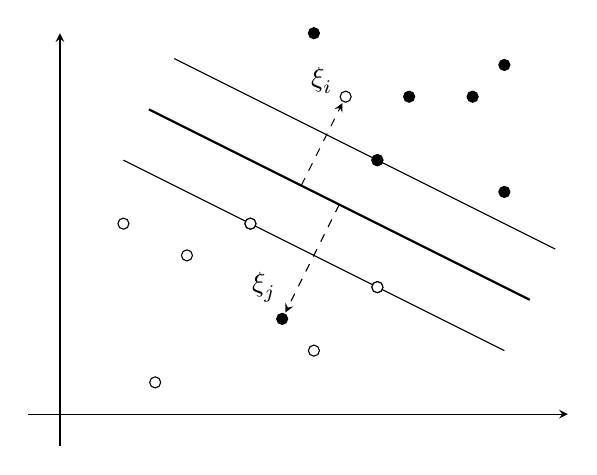
\begin{tikzpicture}
    \begin{axis}[%
      axis equal image,
      axis lines=center,
      xmax = 8,
      xmin = -0.5,
      ymax = 6,
      ymin = -0.5,
      xtick = \empty,
      ytick = \empty,
      no markers]

      % Hiperplanos
      \addplot[black, thin,  domain=1:7]          {(9 - x) / 2};
      \addplot[black, thick, domain=(7/5):(37/5)] {(11 - x) / 2};
      \addplot[black, thin,  domain=(9/5):(39/5)] {(13 - x) / 2};

      % Hiperplano a vectores
      \addplot[dashed, ->] coordinates {(3.8, 3.6) (4.45, 4.9)}
        node[above left]{$\xi_{i}$};
      \addplot[dashed, ->] coordinates {(4.4, 3.3) (3.55, 1.6)}
        node[above left]{$\xi_{j}$};

      \addplot[
        scatter,
        only marks,
        point meta=explicit symbolic,
        scatter/classes={
          a={mark=*},
          b={mark=*, draw=black, fill=white}
        }]
        table[meta=label] {
          x   y   label
          4   6   a
          5   4   a
          5.5 5   a
          6.5 5   a
          7   3.5 a
          7   5.5 a
          1   3   b
          1.5 0.5 b
          2   2.5 b
          3   3   b
          4   1   b
          5   2   b
          3   3   b
          5   2   b
          5   4   a
          4.5 5   b
          3.5 1.5 a
      };
    \end{axis}
  \end{tikzpicture}

\end{document}
